% Options for packages loaded elsewhere
\PassOptionsToPackage{unicode}{hyperref}
\PassOptionsToPackage{hyphens}{url}
\PassOptionsToPackage{dvipsnames,svgnames,x11names}{xcolor}
%
\documentclass[
  letterpaper,
  DIV=11,
  numbers=noendperiod]{scrartcl}

\usepackage{amsmath,amssymb}
\usepackage{lmodern}
\usepackage{iftex}
\ifPDFTeX
  \usepackage[T1]{fontenc}
  \usepackage[utf8]{inputenc}
  \usepackage{textcomp} % provide euro and other symbols
\else % if luatex or xetex
  \usepackage{unicode-math}
  \defaultfontfeatures{Scale=MatchLowercase}
  \defaultfontfeatures[\rmfamily]{Ligatures=TeX,Scale=1}
\fi
% Use upquote if available, for straight quotes in verbatim environments
\IfFileExists{upquote.sty}{\usepackage{upquote}}{}
\IfFileExists{microtype.sty}{% use microtype if available
  \usepackage[]{microtype}
  \UseMicrotypeSet[protrusion]{basicmath} % disable protrusion for tt fonts
}{}
\makeatletter
\@ifundefined{KOMAClassName}{% if non-KOMA class
  \IfFileExists{parskip.sty}{%
    \usepackage{parskip}
  }{% else
    \setlength{\parindent}{0pt}
    \setlength{\parskip}{6pt plus 2pt minus 1pt}}
}{% if KOMA class
  \KOMAoptions{parskip=half}}
\makeatother
\usepackage{xcolor}
\setlength{\emergencystretch}{3em} % prevent overfull lines
\setcounter{secnumdepth}{-\maxdimen} % remove section numbering
% Make \paragraph and \subparagraph free-standing
\ifx\paragraph\undefined\else
  \let\oldparagraph\paragraph
  \renewcommand{\paragraph}[1]{\oldparagraph{#1}\mbox{}}
\fi
\ifx\subparagraph\undefined\else
  \let\oldsubparagraph\subparagraph
  \renewcommand{\subparagraph}[1]{\oldsubparagraph{#1}\mbox{}}
\fi


\providecommand{\tightlist}{%
  \setlength{\itemsep}{0pt}\setlength{\parskip}{0pt}}\usepackage{longtable,booktabs,array}
\usepackage{calc} % for calculating minipage widths
% Correct order of tables after \paragraph or \subparagraph
\usepackage{etoolbox}
\makeatletter
\patchcmd\longtable{\par}{\if@noskipsec\mbox{}\fi\par}{}{}
\makeatother
% Allow footnotes in longtable head/foot
\IfFileExists{footnotehyper.sty}{\usepackage{footnotehyper}}{\usepackage{footnote}}
\makesavenoteenv{longtable}
\usepackage{graphicx}
\makeatletter
\def\maxwidth{\ifdim\Gin@nat@width>\linewidth\linewidth\else\Gin@nat@width\fi}
\def\maxheight{\ifdim\Gin@nat@height>\textheight\textheight\else\Gin@nat@height\fi}
\makeatother
% Scale images if necessary, so that they will not overflow the page
% margins by default, and it is still possible to overwrite the defaults
% using explicit options in \includegraphics[width, height, ...]{}
\setkeys{Gin}{width=\maxwidth,height=\maxheight,keepaspectratio}
% Set default figure placement to htbp
\makeatletter
\def\fps@figure{htbp}
\makeatother

\usepackage{amsmath, xparse}
\usepackage{fancyvrb, fvextra}
\usepackage{bm}
\usepackage{svg}
\usepackage{listings}
\usepackage{sectsty}
\usepackage{xifthen, xparse}
\subsubsectionfont{\centering}
\DefineVerbatimEnvironment{Highlighting}{Verbatim}{breaklines,commandchars=\\\{\}}
\lstset{basicstyle=\ttfamily\footnotesize,breaklines=true}
\newcommand\rowop[1]{\scriptstyle\smash{\xrightarrow[\vphantom{#1}]{\mkern-4mu#1\mkern-4mu}}}
\DeclareDocumentCommand\converttorows%
{>{\SplitList{,}}m}%
{\ProcessList{#1}{\converttorow}}
\NewDocumentCommand{\converttorow}{m}
{\ifthenelse{\isempty{#1}}{}{\rowop{#1}}\\}

\DeclareDocumentCommand \rowops{m}
{\;
\begin{matrix}
\converttorows {#1}
\end{matrix}
\; }
\KOMAoption{captions}{tableheading}
\makeatletter
\makeatother
\makeatletter
\makeatother
\makeatletter
\@ifpackageloaded{caption}{}{\usepackage{caption}}
\AtBeginDocument{%
\ifdefined\contentsname
  \renewcommand*\contentsname{Table of contents}
\else
  \newcommand\contentsname{Table of contents}
\fi
\ifdefined\listfigurename
  \renewcommand*\listfigurename{List of Figures}
\else
  \newcommand\listfigurename{List of Figures}
\fi
\ifdefined\listtablename
  \renewcommand*\listtablename{List of Tables}
\else
  \newcommand\listtablename{List of Tables}
\fi
\ifdefined\figurename
  \renewcommand*\figurename{Figure}
\else
  \newcommand\figurename{Figure}
\fi
\ifdefined\tablename
  \renewcommand*\tablename{Table}
\else
  \newcommand\tablename{Table}
\fi
}
\@ifpackageloaded{float}{}{\usepackage{float}}
\floatstyle{ruled}
\@ifundefined{c@chapter}{\newfloat{codelisting}{h}{lop}}{\newfloat{codelisting}{h}{lop}[chapter]}
\floatname{codelisting}{Listing}
\newcommand*\listoflistings{\listof{codelisting}{List of Listings}}
\makeatother
\makeatletter
\@ifpackageloaded{caption}{}{\usepackage{caption}}
\@ifpackageloaded{subcaption}{}{\usepackage{subcaption}}
\makeatother
\makeatletter
\@ifpackageloaded{tcolorbox}{}{\usepackage[many]{tcolorbox}}
\makeatother
\makeatletter
\@ifundefined{shadecolor}{\definecolor{shadecolor}{rgb}{.97, .97, .97}}
\makeatother
\makeatletter
\makeatother
\ifLuaTeX
  \usepackage{selnolig}  % disable illegal ligatures
\fi
\IfFileExists{bookmark.sty}{\usepackage{bookmark}}{\usepackage{hyperref}}
\IfFileExists{xurl.sty}{\usepackage{xurl}}{} % add URL line breaks if available
\urlstyle{same} % disable monospaced font for URLs
\hypersetup{
  colorlinks=true,
  linkcolor={blue},
  filecolor={Maroon},
  citecolor={Blue},
  urlcolor={Blue},
  pdfcreator={LaTeX via pandoc}}

\author{}
\date{}

\begin{document}
\begin{titlepage}

    \newcommand{\HRule}{\rule{\linewidth}{0.5mm}}
    
    \center
    
    \textsc{\LARGE GSMST }\\[0.3cm]
    \textsc{\Large Applications of Linear Algebra }\\[0.3cm]
    \textsc{\Large in Programming}\\[0.5cm]
    
    \HRule \\[0.4cm]
    { \huge \bfseries Error Correcting Lab}\\[0.03cm]
    \HRule \\[1.5cm]
    
    \begin{minipage}{0.4\textwidth}
    \begin{flushleft} \large
    \emph{Submitted By:}\\
    Anish Goyal \\4th Period
    \end{flushleft}
    \end{minipage}
    ~
    \begin{minipage}{0.4\textwidth}
    \begin{flushright} \large
    \emph{Submitted To:} \\
    Mrs. Denise Stiffler\\Educator
    \end{flushright}
    \end{minipage}\\[1cm]
    
    {\large May 8, 2023}\\[1cm]
    
    
\includegraphics{logo.png}\\[1cm]
    \vfill
    \end{titlepage}
\newpage

\ifdefined\Shaded\renewenvironment{Shaded}{\begin{tcolorbox}[boxrule=0pt, borderline west={3pt}{0pt}{shadecolor}, frame hidden, breakable, enhanced, interior hidden, sharp corners]}{\end{tcolorbox}}\fi

\renewcommand*\contentsname{Table of contents}
{
\hypersetup{linkcolor=}
\setcounter{tocdepth}{4}
\tableofcontents
}
\newpage{}

\hypertarget{sets-of-linear-combinations-and-geometry}{%
\section{Sets of linear combinations and
geometry}\label{sets-of-linear-combinations-and-geometry}}

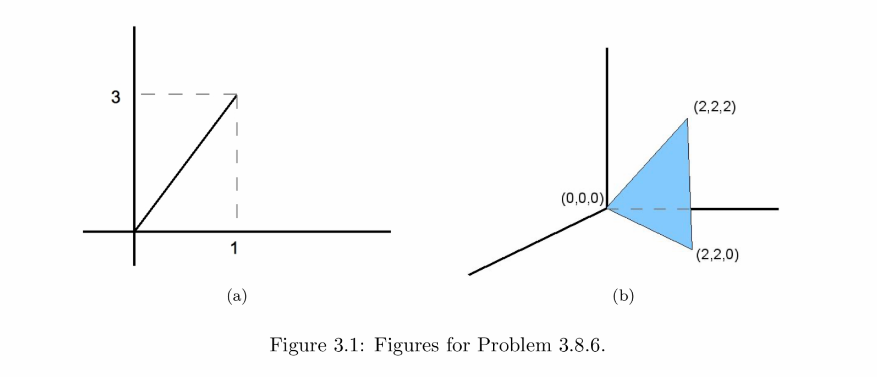
\includegraphics{Figure 3.1.png}

\hypertarget{problem-3.8.6}{%
\subsection{Problem 3.8.6}\label{problem-3.8.6}}

\textbf{Express the line segment in Figure 3.1(a) using a set of linear
combinations. Do the same for the plane containing the triangle in
Figure 3.2(b).}

3.1(a): \(\{\alpha[1, 3], \alpha \in \mathbb{R}, 0 \le \alpha \le 1 \}\)

3.1(b):
\(\{\alpha[2, 2, 2], \alpha \in \mathbb{R}, 0 \le \alpha \le 1 \}\)

\newpage{}

\hypertarget{vector-spaces}{%
\section{Vector spaces}\label{vector-spaces}}

\hypertarget{problem-3.8.7}{%
\subsection{Problem 3.8.7}\label{problem-3.8.7}}

\textbf{Prove or give a counterexample:
``\(\bm{\{[x, y, z] \ : \ x, y, z \in \mathbb{R}, x+y+z=1\}}\) is a
vector space.''}

This is not a vector space because it is not closed under scalar
multiplication. This is because I could multiply the vector
\(v = [1, 0, 0]\), which is a member of the set, by 2. The resulting
vector \(2v = [2, 0, 0]\) is not a member of the set, and therefore it
is not a vector space.

\hypertarget{problem-3.8.8}{%
\subsection{Problem 3.8.8}\label{problem-3.8.8}}

\textbf{Prove or give a counterexample:
``\(\bm{\{[x, y, z] \ : \ x, y, z \in \mathbb{R}, x+y+z=0\}}\) is a
vector space.''}

This is a vector space. The vector contains
\(v_\varnothing \in \mathbb{R}\), and \(0 + 0 + 0 = 0\). This means for
any \(\alpha\) that we multiply \(v\) by, the vector will still be an
element of the set because \(\alpha(0+0+0) \stackrel{\checkmark}{=} 0\),
and it is therefore closed under scalar multiplication. The set is also
closed under vector addition because for any \(u, v\) in the set, it
will always equal 0, since
\(u_1+u_2+u_3+v_1+v_2+v_3 \stackrel{\checkmark}{=} 0\).

\hypertarget{problem-3.8.9}{%
\subsection{Problem 3.8.9}\label{problem-3.8.9}}

\textbf{Prove or give a counterexample:
``\(\bm{\{[x_1, x_2, x_3, x_4, x_5] \ : \ x_1, x_2, x_3, x_4, x_5 \in \mathbb{R}, x_2 = 0 \text{ or } x_5 = 0 \}}\)
is a vector space.''}

This is not a vector space. If we take any vectors \(u\) and \(v\) which
are both members of the set, it is possible that
\(u + v \not \in \{x_2 = 0 \text{ or } x_5 = 0\}\). An example of this
is \(v=[3, 0, 5, 1, 8]\) and \(v=[-2, 3, 4, 9, 0]\). Although both \(u\)
and \(v\) are members of the set, \(u+v\) is not a member of the set
because neither the second or fifth element are zero, which means the
set is not closed under vector addition.

\hypertarget{problem-3.8.10}{%
\subsection{Problem 3.8.10}\label{problem-3.8.10}}

\textbf{Explain your answers.}\\
\textbf{1. Let \(\bm{V}\) be the set of 5-vectors over \(\bm{GF(2)}\)
that have an even number of 1's. Is \(\bm{V}\) a vector space?}

\(V\) is a vector space. \(\forall v \in GF(2), 0v = v_\varnothing\),
which has an even number of 1's, and \(1v = v\), which also has an even
number of 1's per the problem; therefore, it is closed under scalar
multiplication. \(v\) is also closed under vector addition because two
vectors \(u\) and \(v\) in the set will always have the same number of
1's modulo 2.

\textbf{2. Let \(\bm{V}\) be the set of 5-vectors over \(\bm{GF(2)}\)
that have an odd number of 1's. Is \(\bm{V}\) a vector space?}

Any set over \(GF(2)\) with an odd number of 1's is NOT closed under
scalar multiplication and thus cannot be a vector space. This is because
\(\forall v \in GF(2), 0v = [0, 0, 0, 0, 0]\), which has an even number
of 1's (no 1's at all).



\end{document}
